\documentclass{beamer}

%--% Paquetes %----------------------------------%
\usepackage[spanish]{babel}
\usepackage[utf8]{inputenc}
\usepackage[T1]{fontenc}
\usepackage{graphicx}
\usepackage{hyperref}
\usepackage{courier}
\usepackage{listings}
\usepackage{xcolor}
\usepackage{blindtext}
\usepackage{scrextend}
\usepackage[document]{ragged2e}
\usepackage{multicol}
\usepackage{pgfgantt}
\usepackage{minted}
\usepackage{tikz}
\usepackage{longtable}
\usepackage{algorithm}
\usepackage[noend]{algpseudocode}
\usepackage{amsmath}
\usepackage{wrapfig,lipsum,booktabs}
%------------------------------------------------%

%En caso de que LaTeX separe las palabras con - de manera incorrecta, usar
%\hyphenation{deci-sión,e-xa-men, otras palabras....}
\hyphenation{o-cu-rrir}


\usetikzlibrary{positioning,fit,calc}

\makeatletter
\newcommand*{\MoveFitHeight}[1]{%
	\pgfmathsetlengthmacro\fit@inner@sep{%
		\pgfkeysvalueof{/pgf/inner xsep}%
	}%
	\pgfmathsetlengthmacro\fit@text@height{%
		\tikz@text@height
	}%
	\kern-\fit@inner@sep\relax
	\raisebox{\fit@text@height}[0pt][0pt]{#1}%
}
\makeatother

\newcommand{\algTitle}{\textbf{Algoritmo:} }

\newcommand{\bigO}[1]{$O({#1})$}

\usetheme{Berlin}
%\usecolortheme{beaver}

%--% Personal Info %-----------------------------%
\title{Algoritmos de Remoción de Páginas}
\author{Victor Tortolero, 24.569.609}
\institute{
	Sistemas Operativos, FACYT
}
\date{\today}
%------------------------------------------------%


\begin{document}
\setbeamertemplate{caption}{\raggedright\insertcaption\par}

\begin{frame}
	\titlepage

\end{frame}
\author{}


%--% Optimo %---------------------------------------------------------------------%
\begin{frame}
\frametitle{\algTitle Óptimo}

{ \footnotesize
Cada pagina se etiqueta con el numero de instrucciones que se ejecutaran antes de que se referencie. 
La que tenga la etiqueta mas alta se eliminara al ocurrir un fallo de pagina. }

\begin{figure}
	\centering
	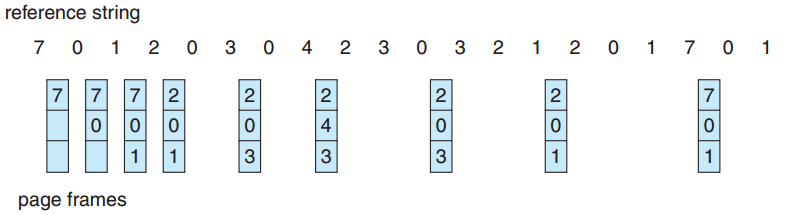
\includegraphics[scale=0.5]{img/optimo.png}
\end{figure}

\end{frame}
%--------------------------------------------------------------------------------%

%--% LRU %---------------------------------------------------------------------%
\begin{frame}
	\frametitle{\algTitle Least Recently Used (LRU)}
	{\scriptsize Descarta la página que no se haya utilizada durante la mayor longitud de tiempo.}
	
	{\footnotesize \textbf{Implementación con Contador}: Con un contador se asocia a cada pagina el tiempo de la ultima vez que se referencio.}
	
	\begin{figure}[H]
		\centering
		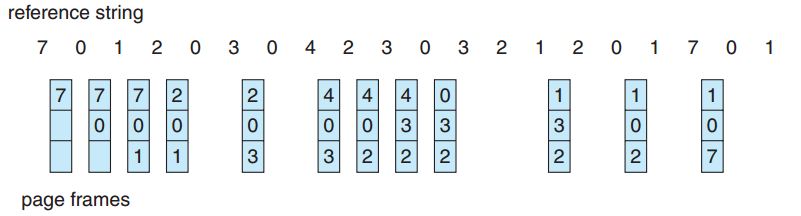
\includegraphics[scale=0.5]{img/lru1.png}
		\caption{Algoritmo LRU con implementado con un contador}
	\end{figure}


\end{frame}

\begin{frame}
	\frametitle{\algTitle Least Recently Used (LRU)}
	{\scriptsize Descarta la página que no se haya utilizada durante la mayor longitud de tiempo.}
	
	{\footnotesize \textbf{Implementación con Pila}: Las paginas mas recientemente referenciadas se mantienen en el tope de la pila, y las menos en el fondo.}
	
	\begin{figure}[H]
		\centering
		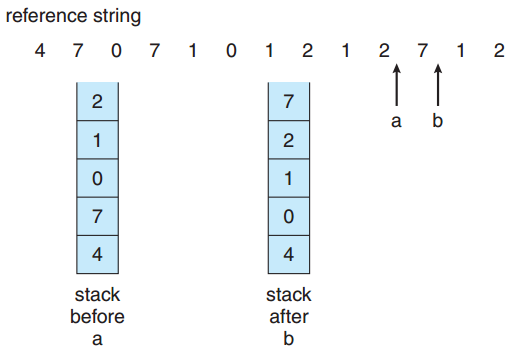
\includegraphics[scale=0.4]{img/lru2.png}
		\caption{Algoritmo LRU implementado con una pila}
	\end{figure}
	
	
\end{frame}
%--------------------------------------------------------------------------------%


%--% FIFO %---------------------------------------------------------------------%
\begin{frame}
	\frametitle{\algTitle First in, First out (FIFO)}
	Se mantiene una lista de las paginas. Al ocurrir un fallo de pagina, se elimina la pagina que esta en la parte frontal y la nueva página se agrega a la parte final de la lista.
	
	\begin{figure}[H]
		\centering
		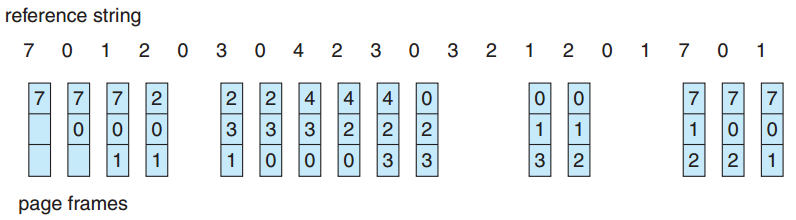
\includegraphics[scale=0.5]{img/fifo.png}
		\caption{Algoritmo FIFO}
	\end{figure}
	
	
\end{frame}
%--------------------------------------------------------------------------------%


%--% Segunda Oportunidad %---------------------------------------------------------------------%
\begin{frame}
	\frametitle{\algTitle Segunda Oportunidad}
	\footnotesize	
	Se revisa la pagina que esta al frente de una lista, y:
	\begin{itemize}
		\footnotesize
		\item Si $R = 0$, la pagina se substituye de inmediato.
		\item Si $R = 1$, se pone en 0, y la pagina se pasa al final de la lista como si acabara de llegar a memoria y sigue buscando.
	\end{itemize}
	
	\begin{figure}[H]
		\centering
		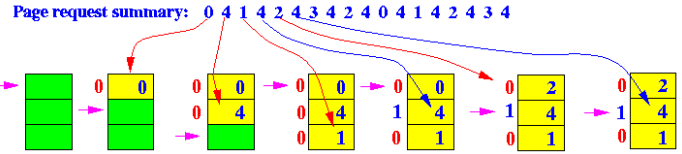
\includegraphics[scale=0.45]{img/sop1.png}
	\end{figure}
	\begin{figure}[H]
		\centering
		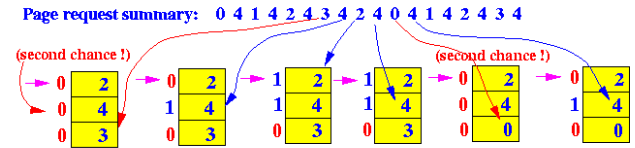
\includegraphics[scale=0.45]{img/sop2.png}
		\caption{Algoritmo Reloj}
	\end{figure}
\end{frame}
%--------------------------------------------------------------------------------%


%--% Reloj %---------------------------------------------------------------------%
\begin{frame}
	\frametitle{\algTitle Reloj}
	\footnotesize
	Las paginas se mantienen en una lista circular, y se apunta a una de ellas.
	\begin{itemize}
		\footnotesize
		\item Si $R = 0$, la pagina se substituye y avanza el apuntador.
		\item Si $R = 1$, se pone en 0, y se avanza el apuntador, y se repite hasta encontrar una pagina con $R = 0$.
	\end{itemize}
	
	\begin{figure}[H]
		\centering
		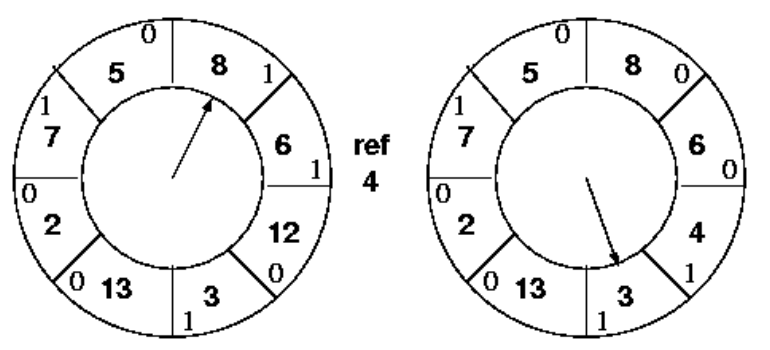
\includegraphics[scale=0.4]{img/reloj2.png}
		\caption{Algoritmo Reloj}
	\end{figure}
\end{frame}
%--------------------------------------------------------------------------------%


%--% NRU %---------------------------------------------------------------------%
\begin{frame}
	\frametitle{\algTitle Not Recently Used (NRU)}
	A cada pagina se asocian 2 bits y se clasifican:
	\begin{itemize}
		\footnotesize
		\item \textbf{Clase 0}: no referenciada, no modificada (R=0, M=0).
		\item \textbf{Clase 1}: no referenciada, modificada (R=0, M=1).
		\item \textbf{Clase 2}: referenciada, no modificada (R=1, M=0).
		\item \textbf{Clase 3}: referenciada, modificada (R=1, M=1).
	\end{itemize}
	 Elimina una página al azar de la clase de menor numeración que no esté vacía.
	

	
\end{frame}
%--------------------------------------------------------------------------------%


%--% Working Set %---------------------------------------------------------------------%
\begin{frame}
	\frametitle{\algTitle Working Set}
	\footnotesize
	Las paginas tienen una edad (tiempo virtual actual menos su tiempo de ultimo uso). Y se tiene un tamaño del conjunto de trabajo.

	\begin{figure}[H]
		\centering
		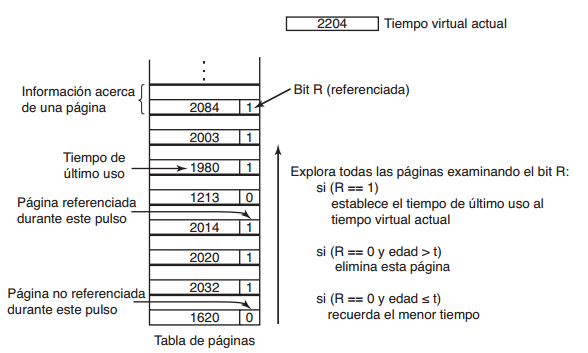
\includegraphics[scale=0.6]{img/workingset.png}
	\end{figure}
\end{frame}
%--------------------------------------------------------------------------------%


%--% WS Clock %---------------------------------------------------------------------%
\begin{frame}
	\frametitle{\algTitle WS Clock}
	\footnotesize
	Mezcla entre el Working Set y el Clock.
	\begin{itemize}
		\footnotesize
		\item Si $R = 1$, se pone en 0 y se avanza el apuntador.
		\item Si $R = 0$ y la edad > $\tau$ y la pagina esta limpia, se coloca en ese espacio.
		\item Si $R = 0$ y la edad > $\tau$ y la pagina esta sucia avanza el apuntador y sigue el algoritmo.
	\end{itemize}
	
	\begin{figure}[H]
		\centering
		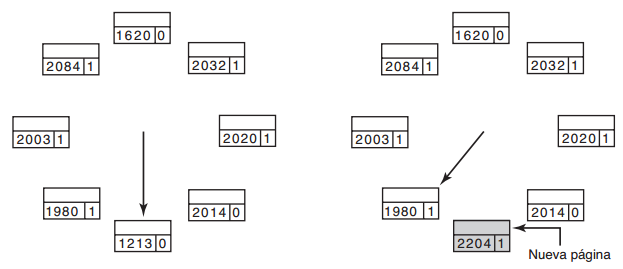
\includegraphics[scale=0.5]{img/wsclock2.png}
		\caption{Algoritmo WS Clock con tiempo virtual actual = 2204}
	\end{figure}
\end{frame}
%--------------------------------------------------------------------------------%


\begin{frame}
	\frametitle{Prediccion de tasa de fallos}
	\footnotesize
	Se denota como $C_{i}$ el numero de veces que aparece $i$. Luego calculamos con la formula 
	
	\begin{equation*}
	F_{m} = \sum_{k=m+1}^{n}C_k + C_\infty
	\end{equation*}
	
	El valor de $F_{m}$ es el numero de fallos de pagina que se presentaran con la cadena de distancias dada y $m$ marcos de pagina. $C_\infty$ es el numero de veces que aparece $\infty$ en la cadena de distancias.
	
	\begin{figure}[H]
		\centering
		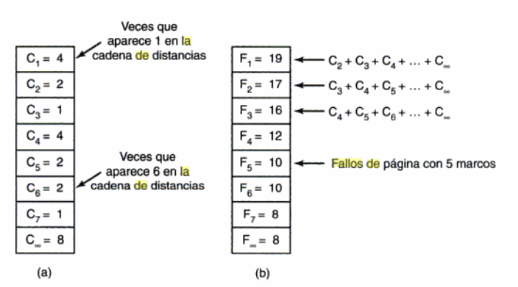
\includegraphics[scale=0.4]{img/fallos.png}
	\end{figure}
\end{frame}



\end{document}